% !TEX root = ../main.tex

% 章标题
\chapter{典型神经网络案例分析}

% 节标题
\section{基于复值神经网络的机器人智能抓取}

% 条标题
\subsection{一类离散时间复值Hopf\/ield神经网络的分析与综合}

% <$x$>为行内公式
假设网络神经元的个数为$n$,其中第$i$个神经元的动态描述为:
% 行间公式环境,此公式环境有自动标号
\begin{equation}
\left\{
\begin{aligned}
	u_i(k+1)&=\sum\limits_{j=1}^nT_{ij}V_{j}(k)+a_iu_i(k)+I_i\\
	V_i(k)&=g_i[u_i(k)]+\intab x\dif x
\end{aligned}
\right.
\end{equation}
其中$u_i(k)\in \mathbb{C},\ V_i(k)\in \mcc$和$I_i\in\mcc$分别为第$i$个神经元在$k$步的状态、输出和阈值,$T_{ij}\in\mcc$为第$j$个神经元到第$i$个神经元的连接权值,$a_i\in\mrr$是第$i$个神经元的动态时间常数,$g(\cdot)$为某种非线性复值函数,即$g_i:\ \mcc\rightarrow\mcc$。

若定义$\mathbf{u}=[u_1,\cdots,u_n]^T\in\mcc^n,\ \mathbf{ V}=[V_1,\cdots,V_n]^T\in\mcc^n,\ \mathbf{g}=[g_1,\ldots,g_n]^T\in\mcc^n\rightarrow\mcc^n,\ \mathbf{ T}
=[T_{ij}]\in\mcc^{n\times n},\ \mathbf{A}=\diag(a_i)\triangleq \diag(A_{ii})
\in\mcc^{n\times n},\ \mathbf{ I}=[I_{i}]\in\mcc^{n}$,则系统动态可写成:
\begin{equation}
\left\{
\begin{aligned}
	\mathbf{u}(k+1)&=\mathbf{T}\cdot\mathbf{V}(k)+\mathbf{A}\mathbf{u}(k)+\mathbf{ I}\\
	\mathbf{V}(k)&=\mathbf{g}[\mathbf{u}(k)]
\end{aligned}
\right.
\end{equation}

如果需要对公式的子公式进行编号,则使用\lstinline{subnumcases}环境:
\begin{lstlisting}
\begin{subnumcases}{\label{w} w\equiv}
	0 & $c = d = 0$\label{wzero}\\
	\sqrt{|c|}\,\sqrt{\frac{1 + \sqrt{1+(d/c)^2}}{2}} & $|c| \geq |d|$ \\
	\sqrt{|d|}\,\sqrt{\frac{|c/d| + \sqrt{1+(c/d)^2}}{2}} & $|c| < |d|$
\end{subnumcases}
\end{lstlisting}
上述代码输出如下:
\begin{subnumcases}{\label{w} w\equiv}
0 & $c = d = 0$\label{wzero}\\
\sqrt{|c|}\,\sqrt{\frac{1 + \sqrt{1+(d/c)^2}}{2}} & $|c| \geq |d|$ \\
\sqrt{|d|}\,\sqrt{\frac{|c/d| + \sqrt{1+(c/d)^2}}{2}} & $|c| < |d|$
\end{subnumcases}

\equref{w}中,\lstinline{label:w}为整个公式的编号,\lstinline{label:wzero}为子公式的编号。

% 条标题
\subsection{一类连续复值 Hopf\/ield 神经网络}

考虑一类复值Hopf\/ield神经网络,该网络具有$n$个神经元,其动态描述如下:
\begin{equation}
\left\{
\begin{aligned}
	\frac{\dif u_i(t)}{\dif t}&=-c_iu_i(t)+\sum\limits_{j=1}^na_{ij}V_{j}(t)+I_i\\
	V_i(t)&=f_i[u_i(t)]
\end{aligned}
\right.
\end{equation}

其中$u_i(t)\in \mathbb{C},\ V_i(t)\in \mcc$和$I_i\in\mcc$分别为第$i$个神经元在时刻$t$的状态、输出和阈值,$a_{ij}\in\mcc$为第$j$个神经元到第$i$个神经元的连接权值,$c_i>0$是第$i$个神经元的动态时间常数,$f(\cdot)$为某种非线性复值函数,即$f_i:\ \mcc\rightarrow\mcc$。

\subsection{一种具有多值状态的复值 Hopf\/ield 神经网络模型}
具有多值状态的复值 Hopf\/ield 神经网络是传统的二值Hopf\/ield 神经网络在复数域的扩展。该网络具有$n$个神经元,单层全连接结构,每个神经元具有复平面单位圆上的$K$种状态,即若表示第$l$个神经元在第$k$步迭代中的状态为$x_l(k)$,则:
\begin{equation}
x_l(k)=\exp[{i\theta_K\cdot l(k)}],\ \theta_K=\frac{2\pi}{K},\ l(k)=0,\ 1,\ \cdots,\ K-1
\end{equation}
 
 \figref{figmulti}给出了状态种类 $K=8$时的神经元状态取值示例,其中状态种类数$K$平分复平面单位圆为$K$等分。当记第$j$个神经元到第$l$个神经元的连接权值为$w_{lj}$时,第$l$神经元在第$k$步迭代后的输出为:
\begin{equation}
y_l(k) = \csign_K\left(\sum\limits_{j=1}^n w_{lj}\cdot x_j(k)\right)
% 公式标签,可用<\eqref{}>引用
\label{eqiter}
\end{equation}
\begin{figure}[!htbp]
	\centering
	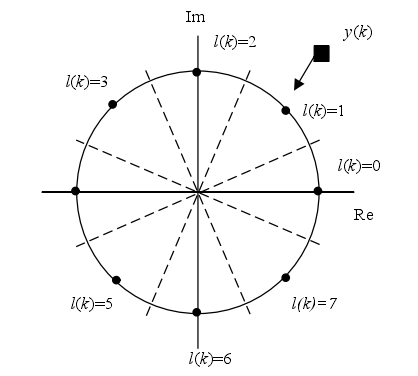
\includegraphics[width=0.5\textwidth]{figmutihopcomplex.png}
	\caption{复值神经元状态$(K=8)$及状态转移规则}
	% 图片标签,可用<\figref{}>引用
     \label{figmulti}
\end{figure}

其中激活函数$\csign(\cdot)$定义如下:
\begin{equation}
\csign(u)=
\left\{
\begin{array}{cc}
	e^{i0},&0\ls\arg[u\cdot\exp(i\pi/K)]<\frac{2\pi}{K}\\
	e^{i\frac{2\pi}{K}},&\frac{2\pi}{K}\ls\arg[u\cdot\exp(i\pi/K)]<\frac{4\pi}{K}\\
	\vdots&\vdots\\
	e^{i\frac{2\pi}{K}(K-1)},&(K-1)\frac{2\pi}{K}
	                                  \ls\arg[u\cdot\exp(i\pi/K)]<2\pi\\
\end{array}
\right.
\end{equation}

可见,激活函数$\csign(\cdot)$实际上可理解为一种复数域上定义的signum函数,它将神经元状态的加权和映射到了复平面单位圆上最接近该加权和的量化点上,其间加权和幅值固定映射成了1。相应的状态转移过程如\figref{figmulti}所示。

从激活函数的定义还可以看出,这种网络是一种全连接回归,且由于神经元的状态有$K$种$(K\gs2)$,因此可将该网络看作传统的二值Hopf\/ield神经网络在复数多值域中的扩展。于是,沿袭Hopf\/ield网络的状态更新方式,该类网络的状态更新也可分同步和异步两种:

异步方式:网络中的神经元状态等概率地依\equref{eqiter}进行更新,一次只更新一个神经元状态;

同步方式:网络的每次迭代中,所有神经元状态同时被更新,即依照下式更新:\begin{equation}
{\mathbf{ X}}(k+1)=\mathbf{ Y}(k)=\csign[\mathbf{ W }\cdot\mathbf{ X }(k)]               
\end{equation}
其中$\mathbf{ X}(k)$为神经元状态$x(k)$组成的列向量,$\mathbf{ W}=(w_{kj})$为整个网络的连接权矩阵。

% 节标题
\section{基于轻量级卷积神经网络的机器人智能抓取}

% 条标题
\subsection{机器人抓取检测的问题描述}

目前基于神经网络的机器人抓取位姿预测方法的研究主要集中在结合基础分类网络如 AlexNet、ResNet 等提高抓取检测准确性上,这些网络最初是为复杂的分类任务和海量数据的特点而设计的,网络结构通常具有大量的参数,需要大量的计算和存储资源。针对上述深度学习抓取检测方法的不足,文献\cite{bib:one}提出了基于 SqueezeNet 的轻量级卷积神经网络抓取预测模型,在不降低准确率的情况下,该网络模型更小,需要的存储资源更少,速度更快,更适合于移动机器人平台中。 类似的设计轻量级模型的工作如\cite{bib11}。

如\figref{figless1}所示的抓取位姿预测问题与如\figref{figless2}所示普通检测问题的区别在于:抓取位姿预测问题不只是在最佳抓取位置处预测出类似于普通检测问题形式的回归框,还要预测出最佳抓取位姿$(x,\ y,\ h,\ w,\ \theta)$。

\begin{figure}[!htbp]
	\centering
	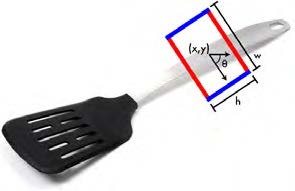
\includegraphics[width=0.4\textwidth]{less1.jpg}
	\caption{五维抓取表示}
     \label{figless1}
\end{figure}
\begin{figure}[!htbp]
	\centering
	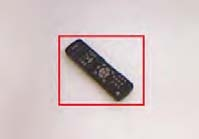
\includegraphics[width=0.3\textwidth]{less2.jpg}
	\caption{普通检测表示}
     \label{figless2}
\end{figure}

机器人抓取位姿检测问题可以被表述为对于给定对象的图像$I$找到最佳抓取位姿$g$。\figref{figless1}显示了一个五维抓取表示\upcite{bib3},以便对物体的潜在的最佳抓取位姿进行表示,五维抓取位姿$g$可以表示为\equref{eqgrasp}:
\begin{equation}
g=f(x,y,h,w,\theta)
\label{eqgrasp}
\end{equation}

其中$(x,\ y)$是与抓取矩形的中心对应的坐标,$h$是平行板的高度,$w$是平行板之间的最大距离,$\theta$是抓取矩形相对于水平轴的取向。蓝线$h$表示二指机器人手爪的平行板,红线$w$对应于抓取之前手爪的平行板之间的距离,该五维抓取表示给出了在对物体执行抓取时平行板夹具的位置和方向。Lenz 等表明一个最佳的五维抓取表示可以被映射回一个可以被机器人用来执行抓取的七维抓取表示,还可以降低计算成本。

% 条标题
\subsection{多模态轻量级抓取检测模型架构}

与以前的方法\upcite{bib3,bib4,bib5}相比,文献\cite{bib:one}使用一个小型轻量级的卷积神经网络架构 SqueezeNet-RM(SqueezeNet Regression Model),该架构结合 SqueezeNet\upcite{bib12}参数少的优点和 DenseNet\upcite{bib13}多旁路连接加强特征复用的思想能提升抓取检测准确率的优点,在康奈尔抓取数据集检测任务上,在保证准确率不降低的情况下,网络模型更小,所需存储空间更少,模型速度更快。

如\figref{figflowchart}所示,整体架构的思想是在 SqueezeNet 网络模型中引入 DenseNet 增加旁路加强特征复用的思想,conv1 和 conv10 之后加入 Batch Normalization,并在最后一层后面添加一个全连接层。全连接层有六个输出神经元对应抓取矩形框的坐标,四个神经元对应位置和高度,抓取角度使用两个附加的参数化坐标:正弦和余弦的两倍角。网络直接从原始图像回归出抓取位姿$(x,y,h,w,\theta)$。

\begin{figure}[!htbp]
	\centering
	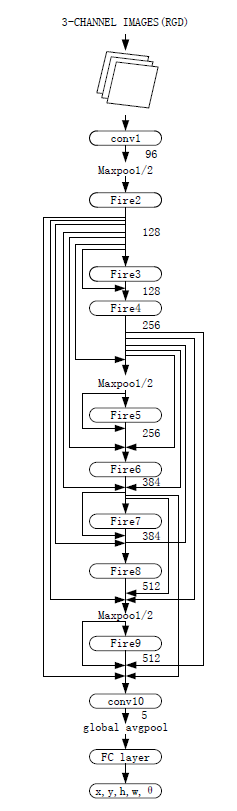
\includegraphics[width=0.4\textwidth]{flowchart}
	\caption{SqueezeNet-RM 网络模型}
     \label{figflowchart}
\end{figure}

% 条标题
\subsection{SqueezeNet轻量级卷积神经网络架构}

如\figref{figflowchart}, SqueezeNet-RM 网络模型以一个独立的卷积层 conv1 为开端,相邻的是 8 个 f\/ire 模块,之后加一个独立的卷积层 conv10,最后以一个最终的全连接层结束。在层 conv1,f\/ire4,f\/ire8 和 conv10 之后使用步长为 2 的 max-pooling、f\/ire2、f\/ire4、f\/ire6 分别向后面的每一层引出旁路连接,这些相对较后的 pooling 和旁路连接有助于提高检测精度。 

类似于 Inception\upcite{bib14}和 DenseNet\upcite{bib15}的模块化思想,SqueezeNet 神经网络采用了模块化的设计思想,它的基础模块称为 f\/ire 模块,如\figref{figfire}所示:  f\/ire 模块含两部分:squeeze 层和 expand 层。首先使用$1\times1$的卷积操作对输入特征图进行压缩,其卷积核数要少于上一层 feature map 数,输出特征图的数量可以远比输入特征图的数量少,这是 squeeze层的设计。然后,采用不同大小的卷积核$1\times1$和$3\times3$进行卷积操作,将这些卷积操作的输出特征图 concat 起来,这是 expand 层操作,最终将特征图的数量提升上去。将上述 f\/ire 模块堆叠, 得到 SqueezeNet 网络。

\begin{figure}[!htbp]
	\centering
	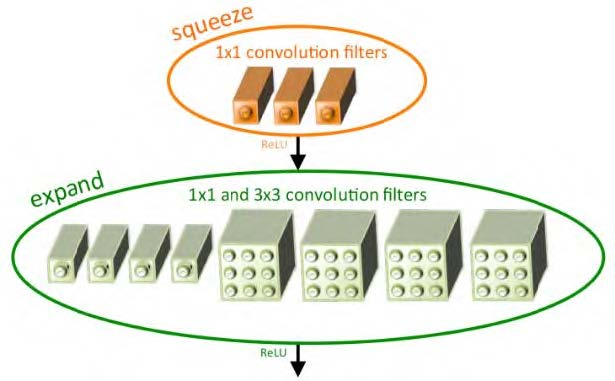
\includegraphics[width=0.6\textwidth]{less3}
	\caption{f\/ire模块}
     \label{figfire}
\end{figure}

SqueezeNet 通过 f\/ire 模块和自身优化结构,采用了以下几种常用的策略实现参数的减少。策略 1: 使用$1\times1$过滤器替换$3\times3$过滤器,因为$1\times1$滤波器具有比$3\times3$滤波器少9倍的参数,见\figref{figfire}中 Squeeze 层。策略 2:使用 Squeeze 层将输入到$3\times3$过滤器的通道的数量减少。具体而言,对于一个完全由$3\times3$滤波器组成的卷积层,该层中的参数的总量是(输入通道的数量)$\times$(滤波器的数量)$\times3\times3$,因此,为了在 CNN 中保持小的参数总数,在采用策略1的同时还要减少$3\times3$滤波器的输入通道的数量。策略 3:延迟降采样, 以使卷积层具有大的激活图,见\figref{figflowchart}中的 Maxpool 位置,大的激活图(通过延迟降采样)可以获得更高的检测精度,有助于提高任务的准确性\upcite{bib16}。策略1和2在试图保持准确性的同时减少CNN中的参数的数量,策略3是在有限的参数运算量上最大化精度。 

文献\cite{bib:one}采用在ImageNet分类问题上表现最佳的SqueezeNet (Simple Bypass  Conection) 架构\upcite{bib12}。 SqueezeNet是一个全卷积网络,在f\/ire9 层之后添加了一个随机失活层dropout\upcite{bib17},以避免过拟合,在 SqueezeNet 网络的最后一层添加一个全连接层Fully Connected Layer (FC层) 作为输出层。

% 节标题
\section{基于级联卷积神经网络的机器人智能抓取}

% 条标题
\subsection{机器人抓取检测的问题}

机器人抓取检测问题包括 2 个部分:抓取位置确定和抓取姿态估计。传统的位置检测方法根据二值化的图像计算物体重心作为抓取位置,但是可抓取位置不在重心处的物体甚多。通常采用滑动窗口法\upcite{bibb6,bibb7} 解决抓取点不在重心上的问题,但此方法以遍历搜索获得最优解,时间代价大。文\cite{bibb8} 对此作出了改进,通过缩小搜索区域范围并减少搜索窗旋转次数来实现时间的优化。Pinto 等人\upcite{bibb9}尝试用随机采样法缩短定位时间,但检测结果因依赖采样位置而表现不稳定,且计算时间减少的成效不明显。 在抓取姿态估计方面,文\cite{bibb7,bibb10}将最优搜索窗的旋转角度作为抓取角度,文\cite{bibb9} 率先以旋转角度为标签将抓取检测感知部分当作分类问题解决,但这些属于粗估计方法,低精度的抓取角度可导致机器人在实际抓取时因受力点错误而抓取失败。因此,减少抓取定位时间消耗和提升姿态估计精度是机器人在线抓取检测时亟待解决的 2 个问题。

深度神经网络用于机器人抓取位姿检测的另一个问题是,已有公开模型如文\cite{bibb7}和文\cite{bibb11}所提出的模型等都是在封闭大数据集上训练所得,通常需要随机器人部署而扩展关于实际特定抓取对象的小样本数据集。迁移学习为特定任务小样本集下深度网络模型训练提供了方法。自建的数据集规模虽小,但能够在已经过百万级封闭数据集训练并具有基本特征提取能力的模型上微调训练,令在特定小样本集下训练的模型仍具有卓越的性能。这样不仅能缩短训练周期,还可提升整个系统的拓展性。

文献\cite{bib:three}针对任意姿态的未知不规则物体,提出一种适于顶抓策略的平面抓取位姿快速检测方法,其主要研究内容及贡献包括:

% enumerate,有序列表环境
% fullwidth,正文不缩进
% label,设置编号格式,可选:\Alph \alph \Roman \roman 或 \arabic
% itemindent,编号缩进量
\begin{enumerate}[fullwidth, label=(\arabic*), itemindent=2em]
\item 提出一种抓取姿态细估计的卷积神经网络模型 Anlge-Net。

\item 在此基础上,提出一种两阶段级联式抓取位姿检测模型。模型第 1 阶段先以基于区域的全卷积网络\upcite{bibb12}为基础提取少量且可靠的候选抓取位置, 再对候选结果筛选排序确定最优抓取位置,以此加快检测速度;第 2 阶段为 Angle-Net 在前一阶段输出的局部位置图像下计算抓取角度。 相比于文\cite{bibb9}的方法,直接计算的抓取角度误差更小,抓取检测精度得以提升。
\end{enumerate}

% 条标题
\subsection{机器人抓取问题描述}

机器人平面抓取作业任务如\figref{figgrasp}所示。机器人视觉系统分析给定抓取场景的彩色图像,推断出顶抓策略下的目标物体最优抓取位姿。

\begin{figure}[!htbp]
	\centering
	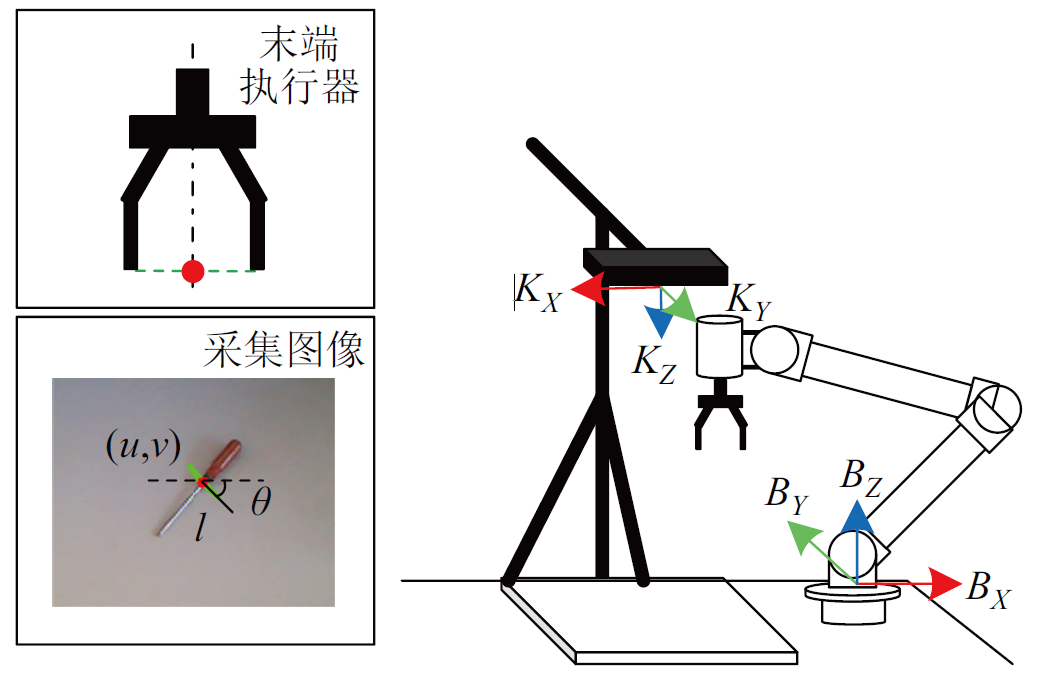
\includegraphics[width=0.6\textwidth]{3grasp}
	\caption{机器人抓取作业任务示例}
     \label{figgrasp}
\end{figure}

为使抓取检测结果与机器人末端执行器位姿对应,图像中抓取位姿检测结果采用基于文\cite{bibb4}方法简化得到的“点线法”表示,如\figref{figgrasp}中的采集图像部分所示,圆点为抓取位置的中心点,图像坐标系下记作$(u, v)$,对应机器人末端执行器两指连线的中点;短实线对应机器人末端执行器的两指连线,抓取角度$\theta$为该线顺时针旋转时与图像坐标系下$X$轴正方向的夹角,对应机器人末端执行器绕机器人 基坐标系$Z$轴旋转的角度。考虑到抓取角度的对称性,设$\theta\in [0, 180)$。线长$l$对应机器人末端执行器尝试抓取时的两指开度。

针对上述研究目标和相关定义,机器人抓取检测问题可描述如下:$t$时刻机器人获取目标的$n$维度特征序列$X (t) = (x_1(t), x_2(t),\cdots, x_n(t))$,有
\begin{equation}
G(u(t), v(t), \theta(t), l(t)) = F(X (t))
\end{equation}

其中,$F$为级联机器人平面抓取位姿检测模型,$G$为“点线法”表示的抓取检测结果。

% 条标题
\subsection{R-FCN与Angle-Net级联的抓取检测器}

抓取位姿检测任务包括抓取点确定和抓取姿态估计 2 个阶段。采取由粗到细的方式,针对各部分任务设计对应的卷积神经网络,并将网络级联成最终的检测模型。

模型结构如\figref{figpoe}所示,第 1 个阶段可视作定位与分类问题,以 R-FCN 为基础实现抓取定位以及抓取角度的粗估计;第 2 个阶段转换成回归问题,通过构造 Angle-Net 模型实现抓取角度的精细估计。

\begin{figure}[!htbp]
	\centering
	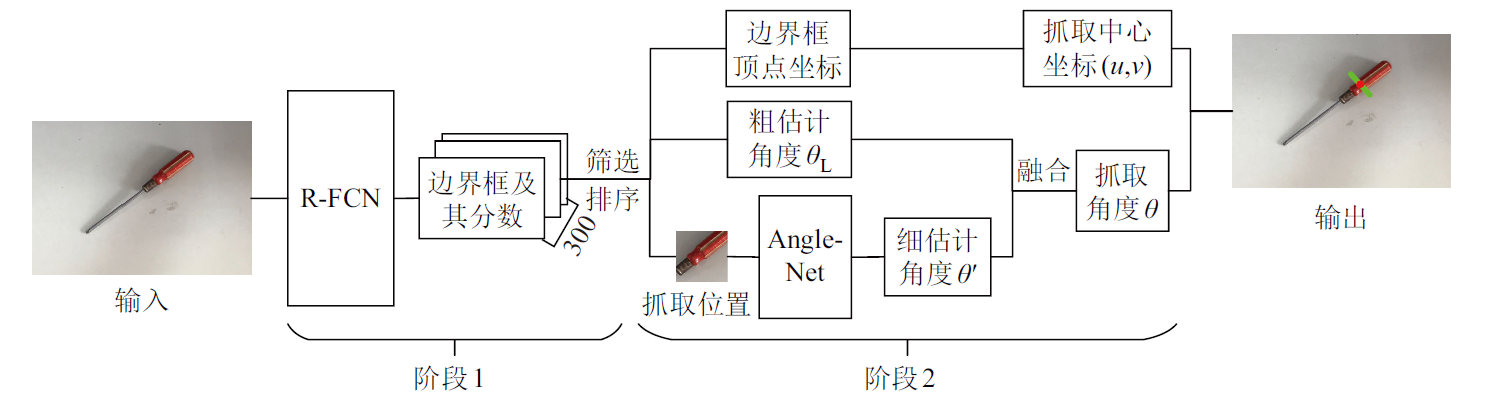
\includegraphics[width=\textwidth]{3posoreest}
	\caption{抓取位姿检测模型结构}
     \label{figpoe}
\end{figure}

针对目标检测问题已提出了许多优秀的深度学习模型,根据文\upcite{bibb14}的研究,基于区域的全卷积网络(R-FCN)兼具优秀的检测速度和准确率。故本文选用 R-FCN 实现图像中候选抓取位置的提取, 可抓取位置在图像上由边界框(bounding-box)标出,抓取点即为边界框中心点.为实现抓取角度的 粗估计,以抓取角度$\theta$为分类标签,共计 4 类:$0\degree,\ 45\degree,\ 90\degree,\ 135\degree$。为在提高检测速度的同时尽量降低对检测结果的影响,抓取位置候选框定为 300 个。 R-FCN 模型输入为任意尺寸的包含目标物体的场景图像,输出为候选框及其对应的可靠性分数,通过筛选和排序确定在工作区域内分数最高的抓取位置。

深度网络目标检测模型根据感兴趣区域(RoI)池化层分为两大类:一类是共享计算的全卷积子网络模型,如 R-CNN\upcite{bibb15}、 快速 R-CNN\upcite{bibb16}、 更快 R-CNN \upcite{bibb17};另一类为不共享计算的作用于各自 RoI 的子网络模型,如 SSD (single shot multibox detector)\upcite{bibb18}、YOLO (you only look once) \upcite{bibb19}。R-FCN 基于 R-CNN 的框架,即先进行区域建议再进行区域分类的策略,为了使检测能对目标的平移做出准确 响应,采用全卷积网络(FCN),用专门的卷积层构建位置敏感分数图 (position-sensitive score map)。每个空间敏感地图对 RoI 的相对空间位置信息进行编码,并在 FCN 上面增加 1 个位置敏感的RoI池化层来监管这些分数图。R-FCN 的结构如\figref{figrfcn}所示。

\begin{figure}[!htbp]
	\centering
	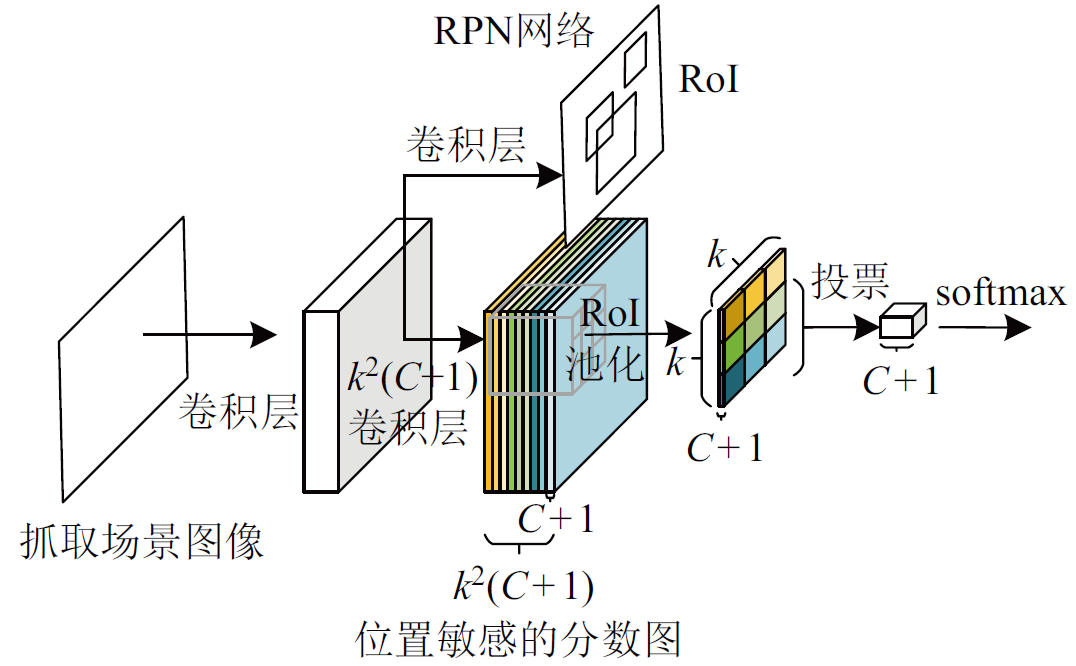
\includegraphics[width=0.6\textwidth]{3rfcn}
	\caption{R-FCN 模型结构}
     \label{figrfcn}
\end{figure}

设待检测类别共有$c$类,在机器人抓取检测模型中$c = 4$。R-FCN 结构中的基础卷积网络基于残差网络(ResNet)\upcite{bibb20},采用 ResNet 的前 100 层并在其最后接一个$1\times1\times1024$的全卷积层。基础卷积网络用于特征提取并输出特征图。区域建议网络沿用更快R-CNN中的区域建议网络(region proposal network,RPN)\upcite{bibb17}网络,生成多个 RoI,即抓取位置候选区域,每个 RoI 被分成$k\times k$块。$k^2$位置敏感分数图作为 R-FCN 中的最后一层卷积层,其功能是输出用于分类的结果。R-FCN 中对RoI 的$(i, j)$块$(0\ls i, j\ls k-1)$进行位置敏感的池化操作,定义为\equref{eqrcijt}:
\begin{equation}
r_c(i,j\mid\theta)=\sum_{(x,y)\in(i,j)}\frac{z_{i,j,c}(x+x_0,\ y+y_0|\Theta)}{n}
\label{eqrcijt}
\end{equation}

其中,$r_c(i,j\mid\theta)$表示$ (i, j) $块对第$ C $类的池化响应;$z_{i,j,c}$是 $k^2(4 + 1)$分数图中的一个,$(x_0, y_0)$ 表示 RoI 的左上角;$n$表示的是每一块当中的像素值,$\Theta$为待学习参数。

池化操作后输出$k^2$个位置敏感的分数图,利用\equref{eqrc}和\equref{eqsc}得到每一类最终的分数,用于计算损失。
\begin{equation}
r_c(\Theta)=\sum_{i,j}r_c(i,j\mid\theta)
\label{eqrc}
\end{equation}
\begin{equation}
s_c(\Theta)=\dfrac{\exp[{r_c(\Theta)}]}{\sum\limits_{c'=0}^C\exp[{r_{c'}(\Theta)}]}
\label{eqsc}
\end{equation}

用模型直接输出角度值替代角度分类标签值可实现更高精度的抓取姿态估计,故构建姿态细估计模型 Angle-Net,结构如\figref{figangle}所示。

\begin{figure}[!htbp]
	\centering
	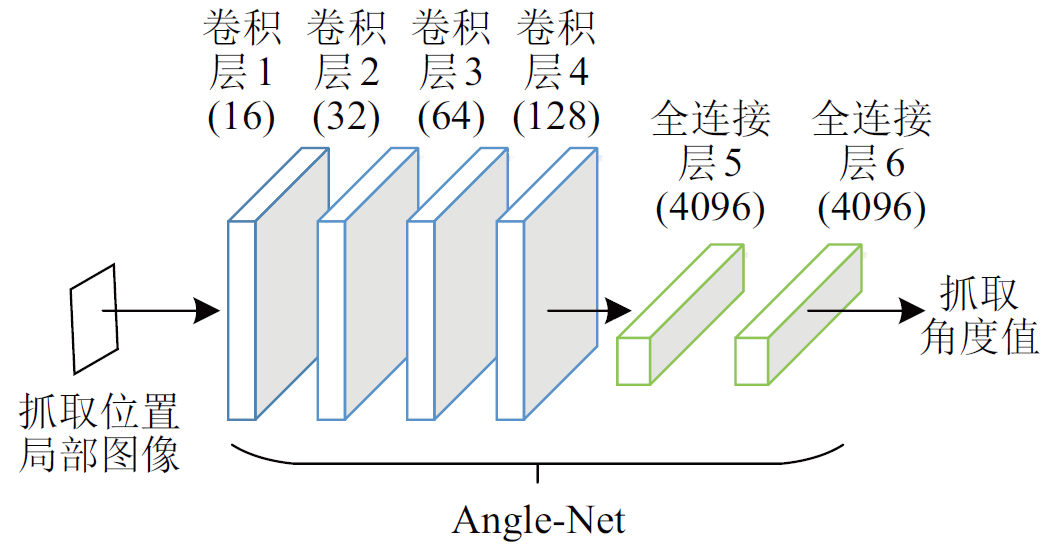
\includegraphics[width=0.6\textwidth]{3angle}
	\caption{Angle-Net 结构}
     \label{figangle}
\end{figure}

Angle-Net 由 4 个卷积层和 2 个全连接层组成。卷积层的卷积核个数分别为 16、 32、 64、 128,全连接层的神经元个数均为 4096。 损失函数(loss function)作为模型预测值与真实值差异程度的估量函数,决定了模型训练的收敛速度和最终效果。 Angle-Net 的损失函数采用L1范数函数,为防止过拟合,在损失函数的基础上加上正则化项,定义如\equref{eqnor}:
\begin{equation}
L=\frac{1}{N}\left(\Big|\theta'-\theta_0\Big|+\sum\limits_i^n\lambda\omega_i^2\right)
\label{eqnor}
\end{equation}
其中,$\theta_0$为期望的抓取角度,$\lambda$为正则化项,$\omega_i$为模型权值参数。

\subsubsection{四级标题示例}

% 条标题
\section{表格绘制示例}

表格按规定为五号字,引用表格示例:\tabref{symbol}.

% 第一列不用填写,自动编号的三线表
% 设置表格第一列计数器归零
\setcounter{rowno}{0}
\begin{center}
\renewcommand{\arraystretch}{1.25}
\begin{table}[H]
\centering %居中
\setlength{\abovecaptionskip}{0pt}
\setlength{\belowcaptionskip}{0pt}
\caption{符号说明}\label{symbol}
\begin{tabular}{>{\stepcounter{rowno}\therowno}ccl}
 \toprule[1.5pt]
\multicolumn{1}{c}{序号}& \makebox[0.2\textwidth][c]{符号}	&  \makebox[0.4\textwidth][c]{意义} \\ \midrule
 &$CNCi\#$&编号为$i$的CNC, $i=1,2,\cdots,8$\\
 &$t_{mj}$    & RGV移动$j$个单位所需时间, $j=0,1,2,3$ \\ 
 &$t_{cnc}$    & CNC加工完成一道工序的物料所需时间 \\ 
 &$t_{cnc1}$    & CNC加工完成第一道工序所需时间 \\ 
 &$t_{cnc2}$    & CNC加工完成第二道工序所需时间 \\ 
\bottomrule[1.5pt]
\end{tabular}
\end{table}
\end{center}

定义定理等环境示例:模板支持以下环境:definition、theorem、proposition、corollary、lemma、remark、exam、exer、note、proof、assumption、conclusion、solution,第二对\{\}内的内容为此定理的label,可以用此label引用,定理\ref{thm:sin}如下。
\begin{theorem}{正弦定理}{thm:sin}
\begin{equation}
\frac{a}{\sin A}=\frac{b}{\sin B}=\frac{c}{\sin C}
\end{equation}
\vspace{0.01cm}
\end{theorem}
% 证明环境
\begin{proof}
以下是一段无意义文字:\lipsum[5]
\end{proof}